\section{Interfaz de Unity}

En esta sección se explicará la interfaz realizada en Unity para el control de los dispositivos usando Unity y ROS2.

\subsection{Uso de NextMind SDK}

El primer objetivo de este proyecto es explorar el uso del dispositivo NextMind en una interfaz gráfica de usuario bidimensional. Esto es importante, porque los ejemplos proporcionados por NextMind están principalmente basados en objetos 3D, y exist\'ian dudas sobre el correcto funcionamiento del API proporcionada por el fabricante en otros contextos como este.

A continuaci\'on se describe la incorporaci\'on a la aplicaci\'on de diferentes elementos del API de NextMind, que conceptualmente fueron descritos en el cap\'itulo dedicado a la tecnolog\'ia empleada.

\subsubsection{NeuroManager}

Para incorporar el NeuroManager, concepto explicado en el apartado \ref{subsection:NeuroManager}, se emplea un ``prefab''. Los prefabs son componentes prefabricados en Unity que permiten reutilizar configuraciones de objetos. Para incorporar el NeuroManager a la escena simplemente se arrastra el prefab correspondiente.



Es importante recalcar que solo puede existir un único NeuroManager activo en un instante dado. Para garantizar que su persistencia a lo largo de las diferentes escenas y evitar su duplicación, se añadió un script llamado DontDestroyOnLoad. Este script verifica si ya existe una instancia de NeuroManager y, en caso afirmativo, destruye cualquier instancia adicional. Si no existe ninguna instancia previa, mantiene la instancia actual en todas las escenas.



El código del script DontDestroyOnLoad es el que se puede ver en el apéndice \ref{appendix:dontdestroyonload}.

\subsubsection{Adición del NeuroTag}
\label{subsubsection:add-neurotag}

Posteriormente, se añadió un botón que contiene un componente NeuroTag, cuyo concepto se explic\'o en el apartado \ref{subsection:NeuroTags}. Gracias a la facilidad de uso de la SDK de Unity, al insertar el componente NeuroTag en un objeto, este permite llamar a una función cada vez que el dispositivo NextMind detecta que el usuario está enfocando su atención en el NeuroTag. Este comportamiento se realiza a través de un disparador (trigger).



Se añadió ese componente arrastrando un prefab de la parte de ejemplos llamada UITag, que es un NeuroTag diseñado para meterlo dentro de un canvas dentro del botón nombrado.



Para configurarlo, se necesita un ``GameObject'' con el script de la función que se desea ejecutar cuando el disparador se active. Una vez que se tiene esto, se arrastra el ``GameObject'' al campo del disparador en la configuración del NeuroTag. Finalmente, en el menú desplegable, se selecciona el método que se desea ejecutar de la clase del script.



Este proceso es válido no solo para los NeuroTags, sino también para otras interacciones como los eventos onClick y similares. Algo relacionado también es que cuando una variable es pública en Unity, puedes asignarle directamente un objeto de la escena (por ejemplo, si es de tipo Text o Image), siempre que este objeto se encuentre dentro de un GameObject.



Se optó por un botón como soporte del NeuroTag por varias razones. En primer lugar, si el NeuroTag falla o no responde, se puede interactuar con el elemento a través del ratón, ya que se le asigna el mismo evento onClick que en el onTrigger del NeuroTag.

\subsubsection{Animación de retroalimentación}

Durante la interacci\'on del usuario con el sistema mediante BCI es esencial que este reciba informaci\'on sobre el nivel de \'exito de la detecci\'on. En caso contrario, no sabr\'ia si su nivel de atenci\'on est\'a siendo adecuado o incluso le puede servir para mejorar su propia t\'ecnica de manejo. 



Para proporcionar una retroalimentación más extensa que la predeterminada (el triángulo central del NeuroTag, véase figura \ref{figure:nextmind-neurotag}), se incorporó la animación que utilizan los NeuroTags en el proceso de calibración. Esta animación emplea un script denominado Flash Controller, al que hay que añadir un ``Flash Animator''.



A continuación, en la jerarquía del botón y a la misma altura que el UITag, se creó un GameObject llamado Background. A este se le añadió un Animator con la animación HaloFeedback, presente en el ejemplo de calibración de NextMind, y también se le incorporó un script llamado NeuroTagFeedback.

\subsubsection{Uso de Flash Controller}

Para manejar la animación de retroalimentación, se incorporó el uso del script Flash Controller proporcionado por NextMind SDK. Este script es responsable de controlar la animación del Background, lo que incluye hacer que un círculo crezca y decrezca, reflejando así el estado del estímulo: crece cuando el estímulo está activo y decrece cuando no lo está.



Primero, se debe asignar el Flash Controller al GameObject que tenga el Animator para la animación de retroalimentación. Para hacer esto, se agrega el script de Flash Controller al GameObject deseado y se configura el Flash Animator en las propiedades del script.



Luego, se debe conectar este Flash Controller al componente NeuroTag. Para hacerlo, se asigna la instancia de Flash Controller al campo correspondiente en las propiedades del NeuroTag. Esto permite que el NeuroTag controle el Flash Controller, activando la animación de crecimiento cuando se detecta un estímulo y la de decrecimiento cuando no.



Este enfoque se basó en el análisis de la estructura del prefab del CircleNeuroTag, el cual incluye un GameObject llamado Background con dos elementos principales: la animación de estímulo y la retroalimentación triangular. Por consiguiente, fue esencial aprender cómo implementar el Background y cómo asignar correctamente el Animator al UITag cuando se agrega el script de Flash Controller.

\subsubsection{Creación del Prefab NeuroButton}

Después de configurar satisfactoriamente un botón con estas características, se decidió convertirlo en un prefab y se le denominó NeuroButton. De este modo, todos los botones con NeuroTags podrían adoptar las mismas características de manera uniforme y sencilla. Para convertir un GameObject en un prefab, el proceso es tan simple como crear un directorio para los prefabs y arrastrar el GameObject hacia ese directorio. El resultado de esta acción se puede ver en la figura \ref{figure:prefab-neurobutton}.

\begin{figure}[!htb]
\centering
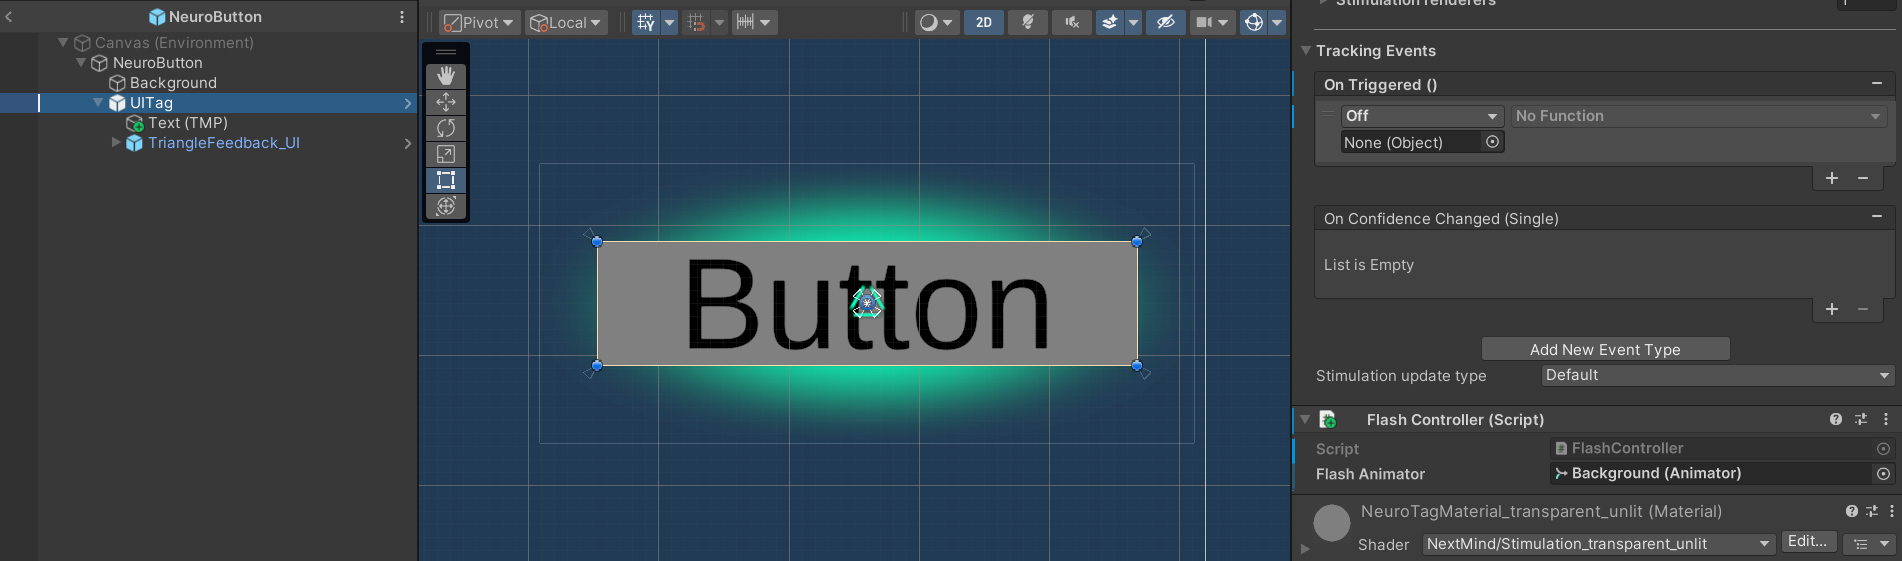
\includegraphics[width=1\linewidth]{figures/prefab-neurobutton.png}
\caption{Prefab del NeuroButton}
\label{figure:prefab-neurobutton}
\end{figure}


\subsubsection{Incorporación de NeuroButtons en la escena}

Una vez creado el prefab de los NeuroButtons, se incorporaron a la escena de Unity. Esto se logró simplemente arrastrando el prefab de cada NeuroButton dentro del canvas de la escena.



Cada NeuroButton se asoció con una dirección específica del pan-tilt: arriba, abajo, izquierda y derecha. Para lograr esto, se asignó a cada botón una función diferente que se activaría al enfocar el NeuroTag correspondiente. Es importante resaltar que, para proporcionar una interacción tanto por interfaz cerebral como por interfaz tradicional (mouse), se asignó la misma función tanto al evento de "onTrigger" del NeuroTag como al evento de "onClick" del botón. De este modo, se puede realizar la misma acción ya sea haciendo clic con el mouse o enfocando con la atención el NeuroTag.



Este tipo de configuración dual permite que el sistema sea operable tanto con el dispositivo NextMind como sin él, proporcionando así un grado de flexibilidad y adaptabilidad en función de las circunstancias del usuario o del ambiente de uso. Además, añade una capa de redundancia que puede resultar útil en caso de problemas técnicos con el dispositivo NextMind o en situaciones en las que el usuario quiera interactuar con el sistema de una manera más tradicional.



Es importante señalar que se encontró un problema común cuando se trabajaba con NeuroTags dentro de un canvas en Unity: los NeuroTags pueden fallar en esta configuración. Este problema está documentado en la página de problemas conocidos y soluciones del SDK de NextMind\cite{NextMindKnownIssues}.



Para solucionar este problema, se cambió el modo de renderizado (Render Mode) del canvas en el Inspector a "Screen - Space: Camera". Posteriormente, se arrastró la cámara principal (Main Camera) de la escena al campo "Render Camera". Este ajuste garantiza que los NeuroTags se renderizan correctamente, permitiendo su detección y activación.

\subsection{Integración de Ros2forUnity con NeuroButtons}

\subsubsection{Prefab de inicialización de ROS2}
Teniendo la instalación realizada del asset Ros2ForUnity (véase el apéndice \ref{ros2forunity}). La integración con NeuroButtons se realizó de la siguiente manera. Se crea un prefab de inicialización de ROS2 que contiene dos scripts: un ROS2 Unity Component, siguiendo la guía oficial de Ros2ForUnity\footnote{Ros2ForUnityUsage: \url{https://github.com/RobotecAI/ros2-for-unity\#usage}}, y Ros2Start, un código que tiene como objetivo crear un nodo que genera un publicador para comunicarse con el Pan-Tilt y un suscriptor para recibir los mensajes del ESP32, sirviendo como canal de comunicación de log (ver ap\'endice\ref{appendix:ros2startscript}) Como este es un script de inicialización, el publicador envía un mensaje a la cámara solicitando su IP si está conectada.



Es relevante destacar que Ros2Start implementa el patrón Singleton, asegurando que, una vez creada la instancia, no se destruye ni se recrea, garantizando un funcionamiento constante incluso durante los cambios de escena. Esta implementación es esencial para mantener la recepción de mensajes del suscriptor, que se discutirá en la sección \ref{subsection:subscriptor}. Igual que Ros2Start, el suscriptor también implementa el patrón Singleton para garantizar la continuidad y coherencia de la gestión de mensajes entrantes.



El patrón Singleton se implementa mediante el uso del método Awake(). Cuando Unity instancie la clase correspondiente, este método será el primero en ejecutarse. Si ya existe una instancia de la clase objetivo (significando que Instance no es nula), el objeto actual se destruirá para asegurar la unicidad de la instancia. En caso contrario, Instance se establecerá como el objeto actual, y gracias a DontDestroyOnLoad(gameObject), la persistencia de este objeto se garantiza a lo largo de los cambios de escena.



Es posible manejar el suscriptor directamente desde Ros2Start, sin embargo, para mantener la claridad y organización del código, se decidió separar esta funcionalidad en un archivo distinto.



Antes de describir el funcionamiento del código, es útil entender los desafíos que presenta la gestión de mensajes entrantes en aplicaciones en tiempo real, como Unity. En un entorno multihilo, múltiples procesos pueden intentar acceder y modificar los datos simultáneamente, potencialmente conduciendo a condiciones de carrera y otros problemas de concurrencia. Para manejar estos desafíos de manera segura y eficiente, se utilizó una cola segura para múltiples hilos (ConcurrentQueue). Esta estructura de datos permite encolar los mensajes a medida que llegan, para luego desencolarlos de manera segura para su procesamiento.

El código completo se encuentra en el apéndice \ref{appendix:ros2startscript}.

Cuando se recibe un mensaje en el tópico "freertos\_header\_log", este se encola para su posterior procesamiento.


Finalmente, en el método Update(), los mensajes se desencolan y se invoca el evento OnMessageReceived para cada uno de ellos.


Esta implementación permite manejar los mensajes de manera segura y eficiente, mitigando los problemas potenciales de concurrencia y optimizando el uso de los recursos. Además, el uso de un patrón de delegado y evento permite una estructura de código flexible y sostenible, ya que los manejadores de eventos pueden ser fácilmente añadidos o eliminados según sea necesario.

\subsubsection{Suscriptor}
\label{subsection:subscriptor}
El componente Ros2SubscriberHandler (véase código en el apéndice \ref{appendix:ros2subscriberhandler}) es el responsable de gestionar y procesar los mensajes recibidos a través del sistema ROS2 en el entorno Unity. Este componente implementa el patrón Singleton, como se ha mencionado anteriormente, lo que garantiza que sólo habrá una única instancia de esta clase durante toda la ejecución del programa.

Cuando se inicializa el Ros2SubscriberHandler, el método Start() se invoca automáticamente para establecer los estados iniciales de las propiedades CameraEnabled, CameraIP y ESP32Enabled. Por defecto, asumimos que no hay ninguna cámara activa, no hay ninguna dirección IP de cámara disponible, y el ESP32 no está habilitado.

El método OnEnable() desempeña un papel esencial en el procesamiento de los mensajes recibidos. Este método se activa cuando el objeto Ros2SubscriberHandler se habilita en la escena de Unity. Dentro de este, se obtiene una referencia al componente Ros2Start y se suscribe al evento OnMessageReceived. Esta suscripción implica que cada vez que se reciba un nuevo mensaje a través de ROS2 (lo que dispara el evento OnMessageReceived), se invocará el método ProcessReceivedMessage.


El método ProcessReceivedMessage es el corazón de la clase Ros2SubscriberHandler. Este es el lugar donde se desglosan y analizan los mensajes entrantes. Cada vez que se recibe un mensaje, el contenido del campo Frame\_id se divide en varias partes. Dependiendo de estas partes, se llevan a cabo diversas acciones, incluyendo la habilitación o deshabilitación de la cámara o del ESP32, y la actualización de la dirección IP de la cámara. El procesamiento de estos mensajes depende del formato y contenido esperado de los mismos en este sistema específico. Por ejemplo, si el mensaje indica que la estación objetivo se ha desconectado, se deshabilita la cámara y se borra la dirección IP de la misma.


\subsubsection{Publicador}
\label{subsubsection:publicador}
El publicador se gestiona en el script Ros2Publish (ver ap\'endince \ref{appendix:ros2publishscript}). En él hay diferentes funciones publicas para su posterior asignación a los NeuroButtons.

Para ello, se ha creado un GameObject que incluye el script Ros2Publish con funciones para publicar, en función de lo que se necesita enviar al suscriptor del ESP32. Este script se diseñó con funciones públicas, lo que permite su asignación a eventos onClick u onTrigger.



En el código publicador que se encuentra en el apéndice \ref{lst:Ros2PublishCode} y el código de la inicialización que se encuentra en el apéndice \ref{lst:Ros2StartCode}, se puede observar que los tipos de mensajes del publicador y del suscriptor son del tipo Header. Header es un tipo de mensaje en ROS2 que contiene metadatos sobre cuándo y cómo se generó la información. Este tipo de mensaje se seleccionó porque proporciona información de control adicional que resulta útil para la depuración.



El mensaje enviado siempre tiene el siguiente formato:

\begin{verbatim}
comando / datos
\end{verbatim}

En este formato, el comando consta de 4 caracteres y los datos tienen un tamaño variable, con un máximo de 100 caracteres definido por el ESP32. Se optó por esta estructura para mejorar la eficiencia, ya que en lugar de tener muchos condicionales if/else, existen unos pocos grupos grandes de if (que corresponden a los comandos), y dentro de esos condicionales if, hay una serie de if/else dependiendo de los datos. Esta división reduce el número de condicionales if/else, mejorando el rendimiento en el peor y en el caso medio.



Para asignar las funciones públicas al onClick y al onTrigger del NeuroButton, hay que añadir a un GameObject el script de Ros2Publish. Este GameObject necesita estar separado del GameObject de inicialización y del suscriptor, porque en el momento que un solo script tenga la opción de 'Don't Destroy', el GameObject entero no se destruye y además si cambiamos de escena, al estar ya creado el Ros2Publish, los NeuroButtons y cualquier cosa que tenga onTrigger u onClick se queda en estado de 'missing'. Por lo tanto, debe construirse al mismo tiempo que el botón o cualquier otro elemento interactivo.



Una vez que se ha añadido a un GameObject que se destruya y construya según se cambia y se vuelve a la escena objetivo, se puede arrastrar ese GameObject al onClick y al onTrigger según corresponda del NeuroButton, y seleccionar la función correspondiente al acto que queremos publicar. Por ejemplo, si estamos en el UpNeuroButton, se publicará el mensaje: % revisar

\begin{verbatim}
"ACT_/Up"
\end{verbatim}


\subsection{Integraci\'on de la cámara}

En esta parte del desarrollo se asume que la c\'amara incorporada al sistema debe funcionar como un servidor web  capaz de realizar un streamming HTTP de im\'agenes, es uno de los requisitos que tiene que tener dicho dispositivo (véase la sección \ref{section:camara}).

Por lo tanto, para integrar la visión de la cámara en Unity, es necesario comprender que la cámara no envía un vídeo continuo, sino que transmite imágenes MJPEG de manera sucesiva. Por tanto, será necesario procesar y separar estos paquetes.



Se procederá a detallar más adelante el proceso de separación y tratamiento de las imágenes. 

\subsubsection{Setup Inicial}
\label{subsubsection:initial-setup}

Se ha creado un Prefab denominado VideoCamera que incluye en su estructura un BackgroundRawImage, un VideoRawImage y un QueryText. La intención de estos elementos es disponer de una imagen de fondo para los momentos en los que no se reciban imágenes de la cámara, un espacio para mostrar las imágenes en directo de la cámara y un área de texto para mostrar el estado de las peticiones GET a la API REST, permitiendo además la visualización de posibles errores en la transmisión.

\subsubsection{Direcciones IP y Puertos}

La cámara utiliza una dirección IP y un puerto específico para el streaming de imágenes, y la misma dirección IP con un puerto distinto para realizar peticiones GET y así poder cambiar su estado en la captura de códigos QR o en el HUD, mediante variables enviadas en la query.

El puerto 81 es utilizado para la visualización del streaming, mientras que el puerto 80 se utiliza para realizar las peticiones GET. 

\subsubsection{Interacción con la Cámara Mediante API REST}
La petición GET para enviar un comando a la aplicación de la cámara se puede ver en el código \ref{lst:GetRequestCamera}.

\begin{lstlisting}[style=basicStyle,label={lst:GetRequestCamera}, caption={Petición get para la cámara}]
http://IP:80/app?app=C&value=V
\end{lstlisting}

Donde IP es la dirección IP del servidor web y C y V funcionan de acuerdo a una tabla específica.

En la tabla \ref{table:cam_commands} se pueden observar los distintos comandos (columna "C") y sus respectivos valores (columna "V") utilizados para las peticiones GET a la cámara. Estos comandos y valores proporcionan una serie de funciones que controlan el estado y la funcionalidad de la cámara, como el reinicio del estado interno de la aplicación, la devolución del estado interno, el establecimiento de dicho estado, el control del streaming, el cambio de modo de detección de QRs, el reinicio del sistema completo y la solicitud de detección de QR. Además, algunos de estos comandos permiten conmutar entre modos de operación dependiendo del valor proporcionado.

\begin{table}[!htb]
\begin{adjustbox}{width=\textwidth,center}
\begin{tabular}{|c|c|c|}
\hline
\textbf{C (comando)} & \textbf{V(valor)} & \textbf{Descripción} \\
\hline
0 & NA & Estado interno: Reinicia el estado interno de la aplicación a 0 \\
\hline
1 & NA & Estado interno: Devuelve el estado interno de la aplicación \\
\hline
2 & s & Estado interno: Establece el estado interno de la aplicación en s \\
\hline
3 & 0 & Control: detiene el streaming \\
\hline
3 & 1 & Control: Cambia el modo de detección de QRs a por petición \\
\hline
4 & NA & Reinicia el sistema completo tras una pausa \\
\hline
5 & 0 & Solicita detección de QR y, si está en modo continuo, la conmuta al modo por petición \\
\hline
\end{tabular}
\end{adjustbox}
\caption{Comandos y valores para peticiones GET a la cámara}
\label{table:cam_commands}
\end{table}

\subsubsection{Escena de Configuración}

Para gestionar todas estas peticiones GET desde Unity, se ha creado una escena adicional denominada "Escena de Configuración" (véase la figura \ref{figure:configuration-scene})

\begin{figure}[!htb]
\centering
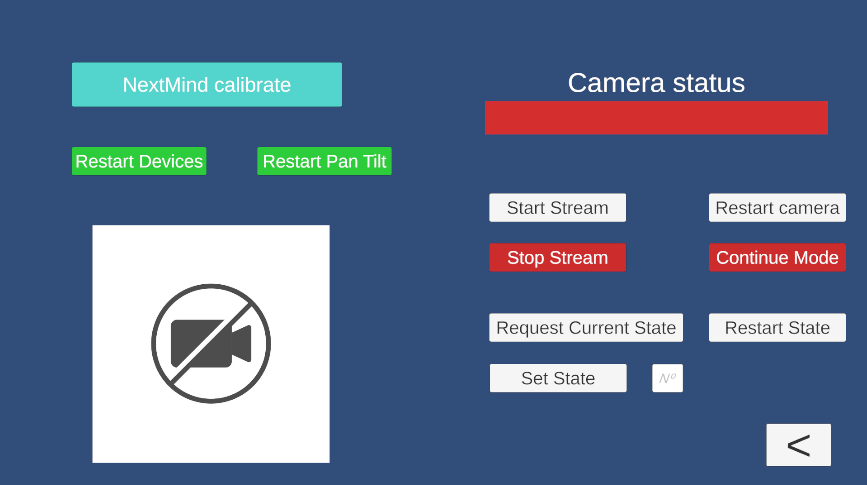
\includegraphics[width=0.8\linewidth]{figures/configuraton-scene.png}
\caption{Escena de configuración}
\label{figure:configuration-scene}
\end{figure}

La funcionalidad de los botones se establece asignando funciones públicas a sus eventos onClick, tal como se detalló anteriormente.

El resultado final en funcionamiento se puede observar en la figura \ref{figure:camera-works-configuration-scene}

\subsubsection{Procesamiento de los Mensajes Recibidos}

Siguiendo un orden lógico, primero se procesan los mensajes que llegan a través del suscriptor, mencionado previamente. En el método ProcessReceivedMessage, estos mensajes se procesan y se almacenan en atributos públicos.

\subsubsection{Clase CameraInfo}

Para mantener una organización y legibilidad óptimas, se creó el script CameraInfo (véase el código en el apéndice \ref{appendix:camerainfoscript}), que es una clase dedicada al estado de la cámara. Esta clase se encarga de recoger la dirección IP de la cámara, si está disponible, y de transformar esa IP en una URL para la captura del streaming o para preparar la URL para la API REST.

Los métodos \lstinline{GetUrl} y \lstinline{GetUrlApiRest} generan las URLs para el streaming de la cámara y para la API REST, respectivamente.

\subsubsection{Clase CameraNetworkCommandController}

Utilizando la clase CameraInfo, pudiendo obtener desde ella el GetUrlApiRest, se pueden hacer peticiones GET añadiéndole la query correspondiente. Eso es lo que trata de hacer este script, para lo que se incluyen métodos públicos con las ordenes descritas en la tabla \ref{table:cam_commands}. El código completo de la clase se puede ver en el apéndice \ref{appendix:CameraNetworkCommandController}.

\subsubsection{CameraNetworkCommandController: Método GetQR}

Como ejemplo de las funciones de la clase CameraNetworkCommandController, el método GetQR es un método público esencial que se encarga de inicializar la solicitud de detección de códigos QR.



El método GetQR es un método público esencial en esta clase, que se encarga de inicializar la solicitud de detección de códigos QR. Primero, limpia cualquier mensaje previo en el campo responseText, que se utiliza para mostrar la respuesta de la cámara. Luego, verifica el estado de la cámara a través del método GetState del objeto cameraInfo. Si la cámara no está habilitada, se interrumpe el proceso, registrando un error en el registro de Unity y en el campo responseText. Si la cámara está habilitada, se construye un comando en formato de cadena de texto ("/app?app=5\&value=0") para solicitar la detección de un código QR. Posteriormente, se registra dicho comando en el registro de Unity para seguimiento y finalmente se inicia una corrutina llamada SendCommand que se encargará de enviar el comando a la cámara.

\subsubsection{CameraNetworkCommandController: Rutina SendCommand}

La rutina SendCommand lleva a cabo la solicitud GET de manera asíncrona, lo que significa que su ejecución se realiza en paralelo al hilo principal de Unity, permitiendo que otros procesos y animaciones sigan funcionando sin interrupciones. En esta rutina, se concatena el comando con la URL base de la API REST de la cámara, proporcionada por el método GetUrlApiRest del objeto cameraInfo, formando así la URL completa de la solicitud GET. Se configura un tiempo de espera de 60 segundos y se envía la petición. Una vez que se recibe la respuesta, se procesa y se muestra en el campo responseText, ofreciendo feedback sobre la operación realizada. En caso de producirse algún error durante la solicitud, se gestiona adecuadamente, proporcionando información detallada sobre la naturaleza del error.



Se modificó el tiempo de espera porque la conexión con la cámara es bastante lenta.

\subsubsection{CameraNetworkCommandController: Método SetState}

El método \lstinline{SetState} tiene un comportamiento un poco diferente, ya que incluye un paso adicional antes de formar y enviar el comando. En este caso, se requiere un valor de entrada proporcionado por el usuario para cambiar el estado de la cámara. Este valor se introduce a través del campo setStateInputField. Se realiza un intento de convertir el texto introducido a un número entero utilizando int.TryParse(). Si la conversión es exitosa, es decir, el usuario ha ingresado un número entero válido, se forma el comando con la estructura "/app?app=2\&value=" + stateValue. Posteriormente, se registra este comando en el registro de Unity y se inicia la corutina SendCommand para enviar la petición a la cámara.



Si la conversión no es exitosa, lo que indica que el usuario ha introducido un valor no válido (no es un número entero), se registra este error en el registro de Unity y se muestra un mensaje de error en el campo responseText.



Por lo tanto, el método SetState extiende la funcionalidad de la clase CameraNetworkCommandController, permitiendo cambiar el estado de la cámara a través de comandos de entrada del usuario, al mismo tiempo que gestiona y proporciona retroalimentación adecuada sobre cualquier error potencial en el proceso.


\subsubsection{Inicialización del Streaming: ImageStreamUrl}
Para inicializar el stream, hay un botón en la escena de configuración como se puede ver en la Figura \ref{figure:configuration-scene}. Ese botón tiene asociado en el evento onClick la función StartStream del script ImageStreamUrl (véase el código completo en el apéndice \ref{appendix:imagestreamurl}) Este script contiene un software de código abierto diseñado para dividir imágenes MJPEG en segmentos manejables para que Unity pueda procesarlos y mostrarlos\footnote{Código abierto para manejar MJPEG en Unity: \url{https://gist.github.com/lightfromshadows/79029ca480393270009173abc7cad858}}.


El método \texttt{StartStream()} es un método público que se utiliza para comenzar a recibir un flujo de imágenes de la cámara. Lo que se ha modificado de este software de código abierto es que primero verifica si la cámara está habilitada utilizando el objeto CameraInfo, y muestra un error si no lo está. A continuación, obtiene la URL de la cámara a través de CameraInfo y comienza a recibir el flujo.



Para hacer esto, StartStream() crea una instancia de Thread para ejecutar el método ReadMJPEGStreamWorker(). Este nuevo hilo se ejecuta en paralelo con el hilo principal del juego de Unity, lo que permite que la recepción y el procesamiento del stream de la cámara se realice sin bloquear la ejecución del resto del juego.



El hilo se inicia con dos argumentos: un identificador único y la URL del stream de la cámara. El identificador único se genera utilizando un número aleatorio para evitar conflictos entre múltiples instancias de ReadMJPEGStreamWorker().

\subsubsection{Procesamiento y Segmentación de la Imagen: ImageStreamUrl}

El método ReadMJPEGStreamWorker() se ejecuta en un hilo separado y se encarga de leer el stream de la cámara. Utiliza el protocolo HTTP GET para solicitar el stream de la cámara desde la URL proporcionada.



A medida que se recibe el stream de la cámara, ReadMJPEGStreamWorker() lo divide en ``frames'' individuales. Cada frame se representa como un array de bytes, y se identifica por una secuencia de bytes específica que marca el inicio y el final de un frame.



Estos frames se añaden a un búfer hasta que se haya recibido un frame completo. Cuando se recibe un frame completo, se envía a Unity para que lo procese y lo muestre. Esto se hace asignando el frame al atributo ``nextFrame'' en el método Update(). Cuando Unity está listo para procesar el siguiente frame, toma el valor de nextFrame, lo procesa y lo muestra, y luego limpia nextFrame.



Si se produce un error al leer el stream de la cámara, ReadMJPEGStreamWorker() intentará reiniciar la conexión hasta un número máximo de intentos.



Por último, el método SendFrame(byte[] bytes) toma un array de bytes que representa un ``frame'' completo y lo convierte en una Texture2D. Si los datos de la imagen son válidos, se aplica a un RenderTexture que puede ser mostrado en Unity. Si los datos de la imagen no son válidos, se muestra un mensaje de error.



Este Texture2D es un atributo público para poder asignarselo desde el inspector.


\subsubsection{Visualización de Imágenes en Unity}

Se dispone de un Texture2D y una imagen de fondo destinada a ser utilizada en el fondo del prefab VideoCamera, ya que son componentes necesarios del mismo. Esta relación se puede observar en la figura \ref{figure:imagestreamurlui-videocameraprefab}. Al atributo BackgroundRawImage se le asigna la imagen de fondo (que debe ser de tipo Sprite) y al atributo VideoRawImage se le asigna el Texture2D, estableciéndose así como la textura del RawImage respectivo.



Para que este Texture2D contenga imágenes, es necesario pasarlas a ImageStreamUrl, que dispone de un atributo público de tipo Texture2D preparado para este propósito. Véase la figura \ref{figure:imagestreamurl}.

\begin{figure}[!htb]
   \centering
    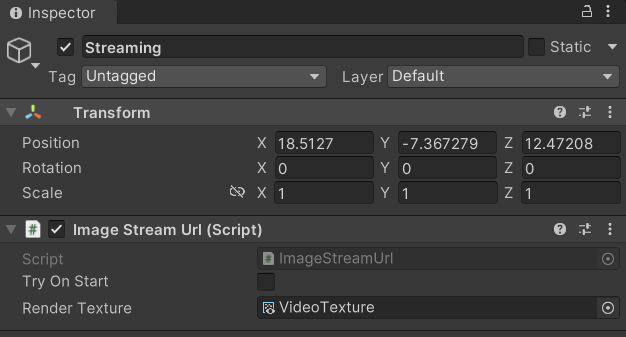
\includegraphics[width=0.75\linewidth]{figures/imagestreamurl.png}
   \caption{ImageStreamUrl en el GameObject Streaming}
   \label{figure:imagestreamurl}
\end{figure}


\subsubsection{Uso del Patrón Singleton en ImageStreamUrl}
Parece razonable que el ImageStreamUrl tenga que mantener su instancia y no poder ser borrada aunque cambiemos de escena para no perder la conexión con la cámara, así que le puse el patrón singleton para que solo existiera una sola instancia del mismo. Se le creó un GameObject único para que no afecte en la persistencia de otros GameObjects y que fuera legible y lógico semánticamente hablando. Ese GameObject se llama Streaming como se puede ver en la figura \ref{figure:imagestreamurl}. Este GameObject se encuentra en la escena principal, donde se encuentran los NeuroButtons.



Gracias a esta configuración, la Textura2D que modifica ImageStreamUrl puede ser utilizada en todas las escenas con la información completamente actualizada. La implementación de este proceso se puede observar en la figura \ref{figure:camera-works-pan-tilt-scene}.

\begin{figure}[!htb]
   \centering
    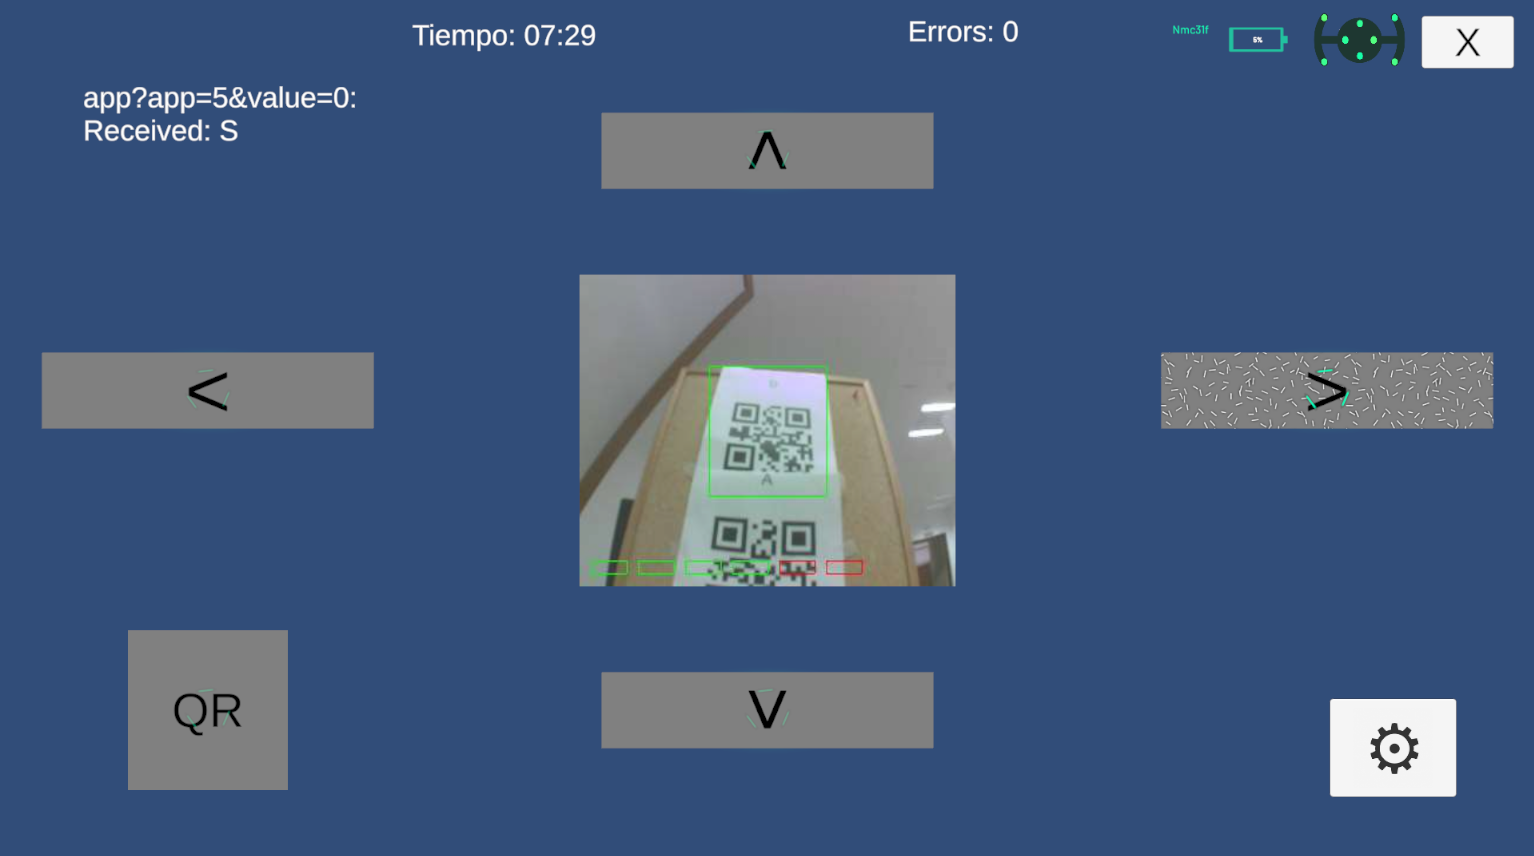
\includegraphics[width=0.8\linewidth]{figures/camera-works-pan-tilt-scene-current.png}
   \caption{Resultado final de la escena de control del Pan-Tilt}
   \label{figure:camera-works-pan-tilt-scene}
\end{figure}

\begin{figure}[!htb]
   \centering
    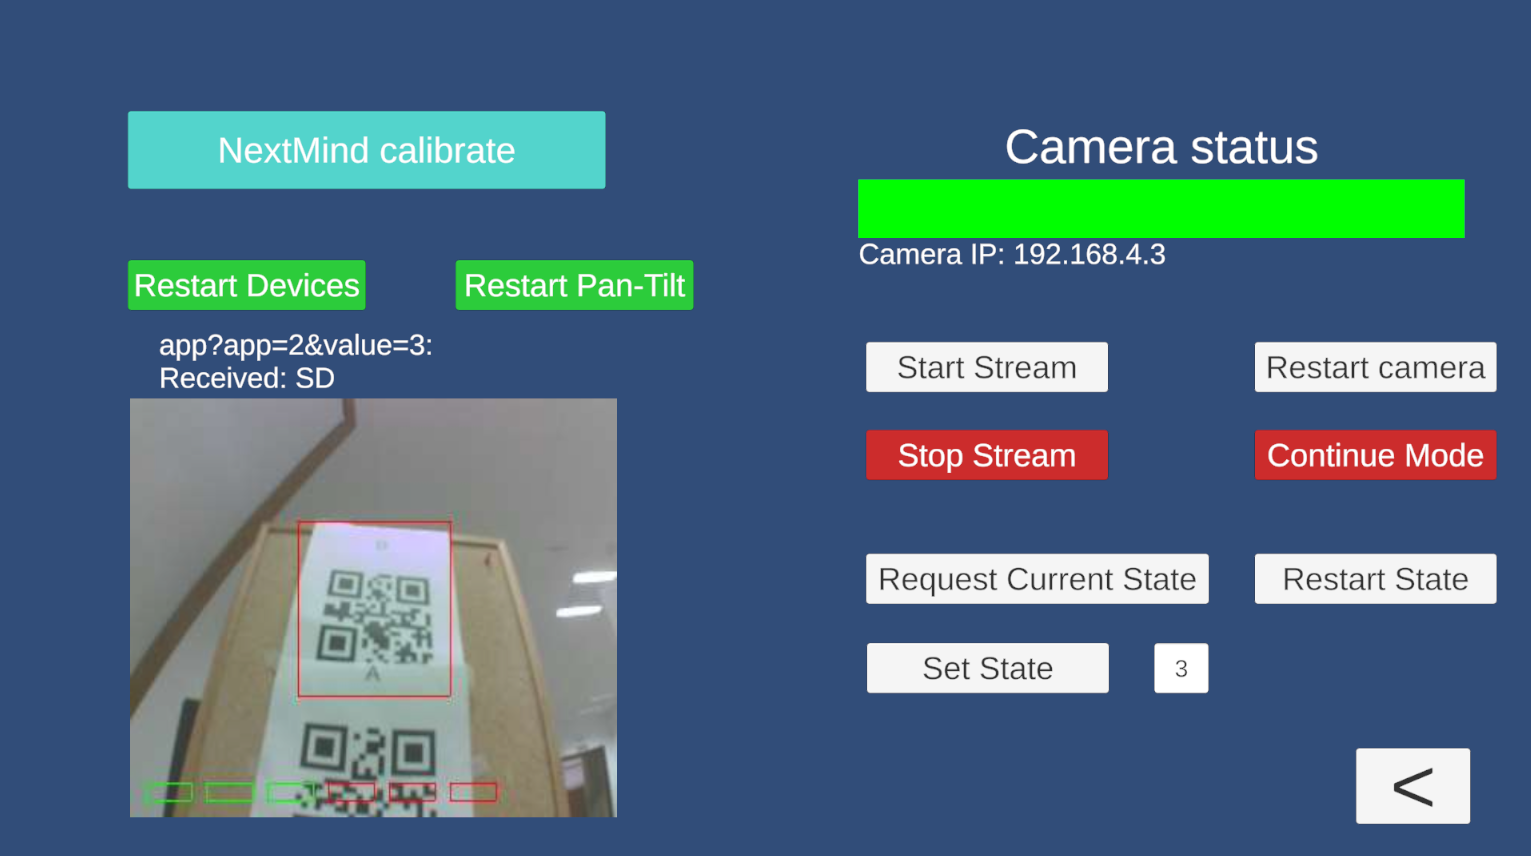
\includegraphics[width=0.8\linewidth]{figures/camera-works-configuration-scene-current.png}
   \caption{Resultado final de la escena de configuración del Pan-Tilt}
   \label{figure:camera-works-configuration-scene}
\end{figure}

\subsubsection{Asignación de CameraInfo y ErrorText: ImageStreamUrlUI}
Dado que el streaming es un objeto persistente, no se puede asignar directamente los valores de CameraInfo y ErrorText desde el inspector en función de la escena, ya que el streaming solo se encuentra en la escena principal y se perdería la referencia al objeto actual si lo asignamos de esa forma.



Para solucionar esto, se ha creado en ImageStreamUrl un método público llamado Initialize. Este método permite asignar los valores de CameraInfo y ErrorText, que son atributos privados, desde otro script que no sea persistente, es decir, que se pueda destruir y repetir en cada escena en la que se quiera mostrar el streaming. De esta forma, cada vez que nos movemos a una nueva escena, estos dos atributos se reasignan, y el objeto siempre sabe qué atributos escoger según la escena.



Se ha creado un nuevo script llamado ImageStreamUrlUI para manejar esta funcionalidad. Este script tiene como atributos públicos una instancia de CameraInfo y un ErrorText, los cuales son asignados a través del inspector. Este script ImageStreamUrlUI se añade al prefab de VideoCamera, lo que resulta en una mejoría de la comodidad de su uso.



De esta forma, el script ImageStreamUrlUI toma la instancia de ImageStreamUrl y, mediante el uso del método público Initialize, asigna los elementos CameraInfo y ErrorText en función de la escena actual (véase figura \ref{figure:imagestreamurlui-videocameraprefab})

\begin{figure}[!htb]
   \centering
    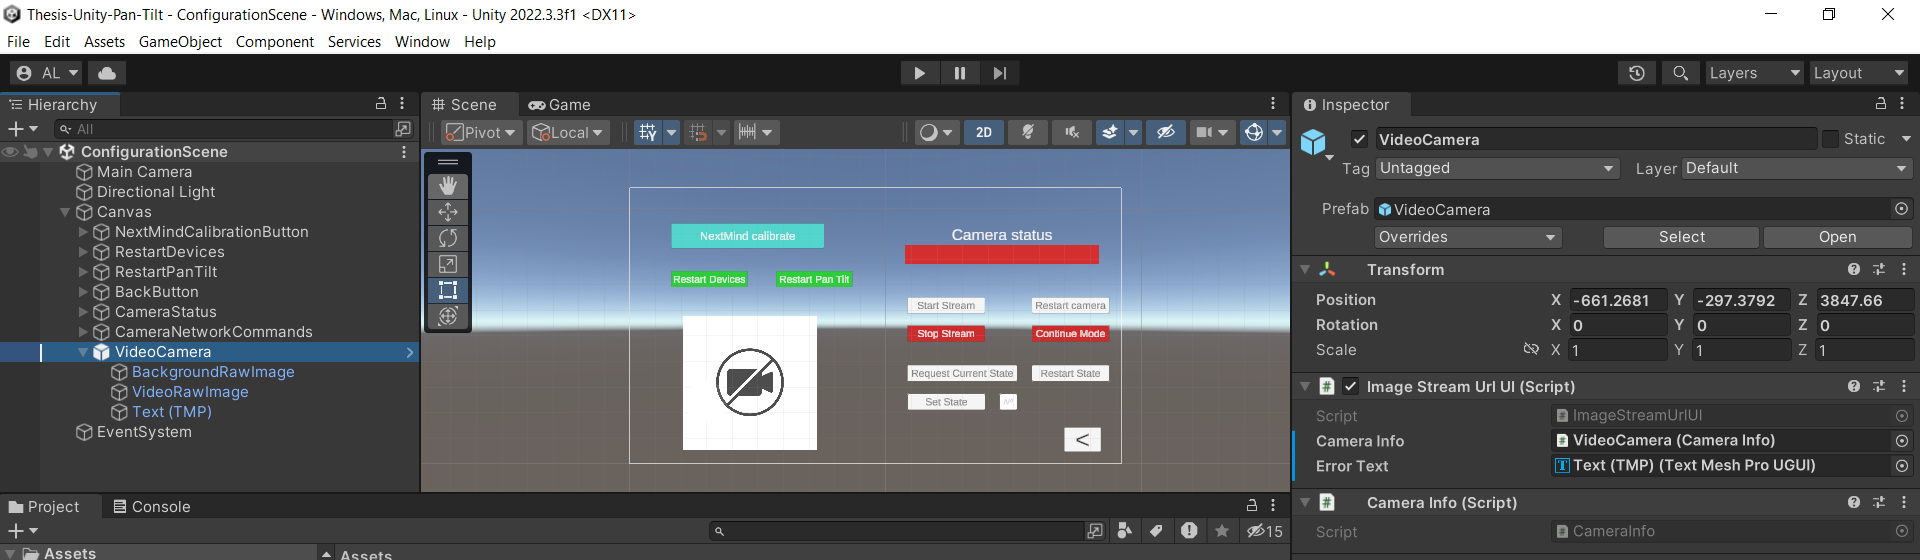
\includegraphics[width=1\linewidth]{figures/imagestreamurlui-videocameraprefab.png}
   \caption{ImageStreamUrlUI en el prefab VideoCamera}
   \label{figure:imagestreamurlui-videocameraprefab}
\end{figure}


\subsection{Botones de Control del Pan-Tilt}
En la escena de configuración quedan dos botones, uno llamado Restart Devices y otro llamado Restart Pan-Tilt.


El botón "Restart devices" aprovecha una peculiaridad en la gestión del WiFi, que actualmente se encuentra fuera del control de micro-ROS. Por lo tanto, no puede ser desconectado internamente, lo que da lugar a un error. Este punto será detallado más adelante en el texto. Cuando ocurre dicho error, se desencadena un reinicio total de todos los dispositivos.

Para implementar esta funcionalidad, recurrimos a un procedimiento previamente utilizado: empleamos el script "Ros2Publish", instanciado en un GameObject en esta escena. Luego, arrastramos ese GameObject al evento onClick correspondiente y seleccionamos la función pública apropiada.

Para obtener una comprensión más detallada de este proceso, se puede referir a la sección \ref{subsubsection:publicador}, donde se explica su funcionamiento.

Se publica el siguiente mensaje:
\begin{verbatim}
CON_/DIS
\end{verbatim}



En el Restart Pan-Tilt también es usando el mismo GameObject que tiene el Ros2Publish en esa escena. Esta vez se usa un comando 

Se publica el siguiente mensaje:
\begin{verbatim}
ACT_/Reset
\end{verbatim}









